\documentclass[sigconf,natbib=true,anonymous]{acmart}
%% WSDM 2027 — snapshot 2026-08-19
%% Main-table GTS-Last/Random: cutoff-fit, no-cross (Beauty wrap_beauty_*; Toys/Grocery wrap_*).
%% tab:early Early row: equal-horizon but not yet matched-protocol (retrain running).
%% tab:loov: Δ only as diagnostic; not GTS-Last.
%% v3.1: expanded for page budget (protocol fig, multi-metric, shift, related, per-seed, RQ3, conclusion, appendix)

\settopmatter{printacmref=false}
\renewcommand\footnotetextcopyrightpermission[1]{}
\setcopyright{none}
\acmConference[WSDM'27]{Proceedings of the 20th ACM International Conference on Web Search and Data Mining}{February 15--19, 2027}{Hong Kong}
\acmYear{2027}
\acmDOI{}
\acmISBN{}

\usepackage{booktabs}
\usepackage{multirow}
\usepackage{amsmath,amssymb}
\usepackage{graphicx}
\usepackage{subcaption}
\usepackage{siunitx}
\usepackage{xspace}
\usepackage{enumitem}
\usepackage{microtype}
\usepackage{balance}
\usepackage{hyperref}

\newcommand{\tfidf}{\textsc{TF-IDF}\xspace}
\newcommand{\llm}{\textsc{LLM}\xspace}
\newcommand{\mv}{\textsc{MV}\xspace}
\newcommand{\base}{\textsc{SASRec}\xspace}

\begin{document}

\title{Do More Text Views Help?\\
A Leakage-Aware Evaluation of Text Representations\\
for Sequential Recommendation}

\author{Anonymous Author(s)}
\affiliation{%
  \institution{Anonymous Institution}
  \country{}}
\renewcommand{\shortauthors}{Anonymous}

%==============================================================================
\begin{abstract}
%==============================================================================
Text features are widely used to enrich sequential recommenders, but comparisons among lexical, single-view LLM, and prompt-based multi-view representations are often conducted under evaluation protocols that permit temporal overlap.
We conduct a leakage-aware controlled study of ID-only, cutoff-fit \tfidf, single-view Qwen2.5-7B, and four-view \llm representations under full-ranking global temporal splitting (GTS) on three Amazon datasets, using GTS-Last as the primary protocol, GTS-Random as a robustness check, and clean leave-one-out (LOO) as a contrast.
Three findings emerge.
First, evaluation protocol changes conclusions: across the evaluated settings, text consistently improves over ID-only on warm targets, but the relative ordering of \tfidf, single-view \llm, and multi-view \llm changes across Last, Random, and LOO, even when Last and Random evaluate the same trained checkpoints.
Second, no text representation is robustly dominant across temporal windows; temporal shift reduces absolute performance while preserving near-ties among text variants.
Third, additional prompt views provide limited marginal value because they are highly redundant: inter-view CKA reaches $0.82$--$0.94$, the concatenated representation uses only $53$--$55\%$ of its nominal effective rank, and leave-one-view-out has negligible downstream effect.
In contrast, \tfidf is geometrically distinct from \llm views (CKA~$\approx 0.19$), suggesting a potentially complementary lexical--semantic axis that is not captured by adding more prompt views.
These results suggest that evaluation protocol and representation redundancy should be diagnosed before attributing gains to increasingly complex LLM text pipelines.
\end{abstract}

\begin{CCSXML}
<ccs2012>
 <concept>
  <concept_id>10002951.10003317.10003347.10003350</concept_id>
  <concept_desc>Information systems~Recommender systems</concept_desc>
  <concept_significance>500</concept_significance>
 </concept>
 <concept>
  <concept_id>10002951.10003317.10003318.10003319</concept_id>
  <concept_desc>Information systems~Content ranking</concept_desc>
  <concept_significance>300</concept_significance>
 </concept>
</ccs2012>
\end{CCSXML}
\ccsdesc[500]{Information systems~Recommender systems}
\ccsdesc[300]{Information systems~Content ranking}

\keywords{Sequential Recommendation, Text Features, Temporal Evaluation, Multi-View Redundancy, Leakage-Aware Protocol}

\maketitle

%==============================================================================
\section{Introduction}
\label{sec:intro}
%==============================================================================

Sequential recommendation predicts a user's next item from historical interactions~\cite{kang2018sasrec,sun2019bert4rec,hidasi2016gru4rec}.
Item text---titles, descriptions, and LLM-generated semantics---is a standard way to enrich ID embeddings and enable cross-domain transfer~\cite{hou2022unisrec,bao2023tallrec}.
A natural working hypothesis is that \emph{richer text always helps}: LLM embeddings should beat bag-of-words, and multiple prompt-based views should beat a single view.

This hypothesis is widely held.
Recent work routinely reports that LLM-generated item descriptions improve accuracy over TF-IDF or Word2Vec features~\cite{hou2022unisrec,bao2023tallrec}, and multi-view prompt strategies are increasingly adopted to capture complementary item facets such as function, audience, and style.
Practitioners building production recommenders face a concrete decision: should they invest in LLM inference and multi-prompt pipelines for text features, or does a lightweight bag-of-words baseline suffice?
The answer depends critically on how the comparison is evaluated---a consideration that is seldom examined in text-enhanced recommendation papers.

This hypothesis rests on fragile evaluation foundations.
Most text-enhanced sequential recommenders are validated with leave-one-out (LOO) splits that, as shown by \citet{ji2023evaluation} and \citet{sun2023reevaluation}, allow temporal overlap between training and test, yielding higher absolute metrics and potentially distorting model comparisons.
In a deployment scenario, a recommender must predict items that a user will interact with \emph{in the future}, not reconstruct a randomly held-out historical interaction.
Global temporal split (GTS) better simulates this deployment constraint, but introduces additional design choices: the \emph{target-selection mode} (Last, Random, Successive, or All interactions per user in the test window) itself changes effective task difficulty and can alter model rankings~\cite{gusak2025time}.
Prior work has studied split effects in general~\cite{meng2020temporal,ji2023evaluation}; we show that these effects are \emph{specifically decisive} for the \tfidf vs.\ \llm vs.\ multi-view comparison.

Text features also require preprocessing---vocabulary construction, IDF weighting, SVD projection, and LLM embedding whitening---each of which must respect the temporal boundary.
If these statistics are computed on the full item set (including future items), the resulting features carry information unavailable at training time, introducing a form of leakage orthogonal to the train/test split itself.
We therefore enforce strict \emph{cutoff-fit} controls throughout: all text preprocessing is fit only on items appearing before the training cutoff.

We conduct this study comparing five model variants on three Amazon datasets under GTS-Last (primary), GTS-Random (robustness check), and clean LOO (contrast), with an Early temporal window and UniSRec~\cite{hou2022unisrec} as external baseline.
We diagnose multi-view behavior with CKA~\cite{kornblith2019cka}, effective rank, and leave-one-view-out (LOOV).

\smallskip\noindent\textbf{Research questions.}
\begin{enumerate}[leftmargin=*,itemsep=1pt]
\item[\textbf{RQ1}] \emph{Protocol effect.}
Do clean LOO, GTS-Last, and GTS-Random change the absolute gains and relative ranking of \tfidf, single-view \llm, and prompt multi-view?
\item[\textbf{RQ2}] \emph{Temporal robustness.}
Can the conclusions drawn under the Main temporal window ($80\%$ cutoff) survive when the training window shrinks (Early, $60\%$ cutoff)?
\item[\textbf{RQ3}] \emph{Multi-view redundancy.}
Why do four prompt views not reliably outperform a single \llm view or even \tfidf, and where does potential complementarity lie?
\end{enumerate}

\smallskip\noindent\textbf{Contributions.}
\begin{enumerate}[leftmargin=*,itemsep=1pt]
\item A leakage-aware comparison on three datasets showing that evaluation protocol changes text-representation rankings.  Within GTS, the same trained checkpoints yield different winners under Last vs.\ Random (\textbf{target effect}); switching from GTS to LOO changes both training data and targets (\textbf{split effect}).  Text consistently beats ID, but \emph{which} text is best is protocol-sensitive.
\item Cross-window evidence that no single text variant dominates: under an equal-horizon Early window ($60\%$ cutoff, same valid/test span), used here as a temporal stress test, absolute MRR drops substantially yet text variants remain within 0.001 of each other.
\item A triangulated redundancy analysis (CKA + effective rank + LOOV) spanning raw 3584-d Qwen hidden states through 64-d post-whitening, jointly explaining limited multi-view gains, while identifying lexical--semantic dissimilarity (TF vs.\ LLM, CKA$\approx$0.19) as a potential complementarity axis.
\end{enumerate}

%==============================================================================
\section{Related Work}
\label{sec:related}
%==============================================================================

\paragraph{Text-enhanced sequential recommendation.}
Early systems fused bag-of-words or review text with collaborative filtering~\cite{wang2015cdl,salton1988termweighting}.
Modern approaches encode titles and descriptions with pretrained language models for cross-domain transfer~\cite{hou2022unisrec,hou2023vqrec,geng2022p5,bao2023tallrec}.
UniSRec learns transferable item representations from text and adapts them via a lightweight MoE~\cite{hou2022unisrec}; VQ-Rec quantizes textual embeddings for transfer~\cite{hou2023vqrec}; P5 casts recommendation as language modeling~\cite{geng2022p5}; TALLRec aligns LLMs to ranking via instruction tuning~\cite{bao2023tallrec}.
These systems typically report LOO or loosely specified temporal protocols.
We do \emph{not} propose a new architecture; we ask whether stronger text encoders and more views remain advantageous once temporal leakage is controlled under a fixed backbone.

\paragraph{LLM-based item representations.}
Beyond architecture papers, a growing practice is to treat LLM embeddings as drop-in item features---either as a single view (title/description) or as multiple prompt-conditioned views that supposedly capture complementary facets (function, audience, style).
This practice is motivated by the intuition that different prompts can elicit diverse semantic aspects of an item (e.g., ``describe the function'' vs.\ ``describe the target audience''), thereby increasing feature coverage.
However, when all views are produced by the \emph{same} pretrained encoder applied to the \emph{same} item text, the diversity of the resulting representations depends on how much the encoder's internal representations actually change in response to different instructions---a question that has received little empirical attention in the recommendation literature.
Our study isolates this representation choice from architectural novelty: the same SASRec backbone and fusion pipeline are held fixed while only the text source changes (\tfidf, single-view \llm, or four-view \llm).

\paragraph{Evaluation protocols and temporal leakage.}
Sampled metrics distort rankings~\cite{krichene2020sampledmetrics}; LOO vs.\ time-based splits change absolute scores and can alter model selection~\cite{ji2023evaluation,sun2023reevaluation,meng2020temporal}.
\citet{hidasi2018recurrent} showed that seemingly minor protocol choices can cause large shifts in relative rankings of sequential models.
Within GTS, target-selection mode matters: \citet{gusak2025time} show that Successive best approximates online next-item prediction but is expensive; Last is a deterministic low-cost proxy; Random has the highest rank-correlation with Successive (we average three sampling seeds because Random is non-deterministic); and All packs multiple items into one ground-truth set, introducing task mismatch and the weakest correlation with Successive.
Beyond sequential recommendation, the impact of temporal protocols has also been documented in session-based~\cite{hidasi2018recurrent} and general collaborative filtering settings~\cite{meng2020temporal}, confirming that protocol sensitivity is not a niche issue but a systemic concern across recommendation paradigms.
We specialize this finding to text representations: protocol changes conclusions \emph{precisely because} \tfidf, \llm, and \mv respond differently to distribution shift.
Matching validation and test target modes (both Last, or both Random) is also recommended for reliable model selection~\cite{gusak2025time}; our Early-window experiments keep this alignment.

\paragraph{Multi-view learning and representation redundancy.}
Multi-view theory holds that views must be \emph{useful and complementary}; more views do not guarantee benefit~\cite{xu2013multiview}.
In computer vision, \citet{kornblith2019cka} introduced CKA (Centered Kernel Alignment) to measure representational similarity of Gram structures across network layers and architectures; it can detect structural redundancy even when instance-level pairwise cosine is moderate or near zero.
In NLP, \citet{ethayarajh2019contextual} revealed that contextual word embeddings from different layers of the same pretrained model are highly anisotropic and occupy a narrow cone in embedding space---a form of geometric redundancy.
Effective rank (entropy of normalized singular values) provides a complementary diagnostic, quantifying how much of a representation's nominal dimensionality is actually used.
These tools have been applied to analyze network depth~\cite{kornblith2019cka} and embedding quality~\cite{ethayarajh2019contextual}, but to our knowledge have not been jointly deployed to diagnose \emph{multi-prompt} redundancy in recommendation.
We combine CKA, effective rank, and LOOV---not any single measure alone---to explain limited multi-view gains.

\paragraph{Information geometry of embeddings.}
Singular-value concentration and anisotropy are known failure modes of pretrained text embeddings~\cite{ethayarajh2019contextual}.
When multiple views are generated from the same encoder, these geometric properties propagate: each view inherits similar spectral structure, and concatenation does not proportionally expand the effective subspace.
Our effective-rank analysis connects this literature to sequential recommendation: concatenating four prompt views that share the same encoder yields ER/dim $\approx$0.53, whereas a lexical \tfidf SVD of the same dimension retains ER/dim $\approx$0.98.

%==============================================================================
\section{Controlled Study Setup}
\label{sec:setup}
%==============================================================================

\subsection{Temporal Protocols}
\label{sec:protocol}

\paragraph{GTS-Last (primary).}
Interactions are globally ordered by timestamp; RecBole's \texttt{TS} split~\cite{zhao2021recbole} with $[0.8,0.1,0.1]$ (Main) or $[0.6,0.1,0.1]$ (Early, equal horizon).
After sequential augmentation, each user contributes only their \textbf{chronologically last} test interaction (one target per user)---the deterministic last-item proxy studied by \citet{gusak2025time}.

\paragraph{GTS-Random (robustness check).}
Same checkpoints; each user contributes one \textbf{uniformly random} test interaction.  We average over three target-sampling seeds (42, 123, 456) for stability; cross-seed std per checkpoint is 0.001--0.003.
Random has the highest rank-correlation with Successive~\cite{gusak2025time} and serves as a cross-check.

\paragraph{Clean LOO (contrast).}
Leave-one-out (last-3 interactions per user as train/valid/test; no time cutoff).
Included only to quantify the protocol gap; \emph{not} used for primary conclusions.

\paragraph{GTS-All (appendix).}
All post-cutoff targets per user; relegated to Appendix~\ref{app:gts-all} due to task-mismatch concerns~\cite{gusak2025time}.

\paragraph{Leakage controls.}
\tfidf vocabulary/IDF, SVD projection, and LLM center/whitening are fit only on items appearing before the training cutoff.
Evaluation filters users with $\ge 5$ training interactions.
Main tables report \textbf{warm-target} results: the test target must belong to the training-time item catalog, which is also the candidate set at inference.
All-target and unseen diagnostics appear in Appendix~\ref{app:alltarget}.

\subsection{Text Representations and Models}
\label{sec:models}

All variants share a \base~\cite{kang2018sasrec} backbone ($d{=}256$, 2 layers, 2 attention heads).

\begin{itemize}[leftmargin=*,itemsep=1pt]
\item \textbf{ID}: ID embeddings only.
\item \textbf{TF}: train-cutoff \tfidf $\to$ SVD 256-d $\to$ lightweight projection head + InfoNCE alignment~\cite{oord2018cpc}.
\item \textbf{LLM}: single-view Qwen2.5-7B~\cite{qwen2024qwen25} item embedding (train-cutoff centered and whitened), same fusion pipeline.
\item \textbf{MV}: four prompt views (Description / Function / Audience / Style) $\to$ per-view 64-d projections $\to$ 256-d concatenation $\to$ shared projection; no cross-attention.
\item \textbf{UniSRec}~\cite{hou2022unisrec}: external text-enhanced sequential baseline with the same TS-whitened LLM embeddings and identical eval filter.
\end{itemize}

TF/LLM/MV use two-phase training: Phase~A (text-head warmup via InfoNCE), then Phase~B (joint BPR~\cite{rendle2009bpr} + InfoNCE fine-tuning).
Hyperparameters for the Early window are frozen from Main (no re-tuning).

\subsection{Datasets}

Amazon Beauty, Toys \& Games, and Grocery \& Gourmet Food~\cite{mcauley2015amazon,ni2019amazon}:
\begin{itemize}[leftmargin=*,itemsep=1pt]
\item \textbf{Beauty}: 1.21M users, 259K items, 2.02M interactions.
\item \textbf{Toys}: 1.28M users, 336K items, 2.25M interactions.
\item \textbf{Grocery}: 768K users, 172K items, 1.30M interactions (same-platform replication; not claimed as domain diversity).
\end{itemize}

\subsection{Evaluation Details}

Full-ranking Hit@10, NDCG@10, MRR@10~\cite{krichene2020sampledmetrics}.
Main tables: MRR@10, mean$\pm$sample-std over 3 seeds (42, 2024, 2026); NDCG/Hit reported as secondary metrics.
All runs on a single NVIDIA RTX 5090; per-model training: 15--65~min.

%==============================================================================
\section{RQ1: Protocol Changes Rankings}
\label{sec:rq1}
%==============================================================================

\begin{table}[t]
\centering
\caption{%
Protocol contrast --- warm-target MRR@10 (3 training-seed mean$\pm$std, min5 filter; GTS-Random additionally averaged over 3 target-sampling seeds).
\textbf{Bold}: best text method per row.
Winners change with protocol: Last favors MV; Random favors TF$\approx$MV (within one std); LOO favors LLM$\approx$MV.%
}
\label{tab:protocol}
\small
\setlength{\tabcolsep}{2.8pt}
\begin{tabular}{@{}llccccc@{}}
\toprule
Dataset & Protocol & ID & TF & LLM & MV & UniSRec \\
\midrule
\multirow{3}{*}{Beauty}
 & GTS-Last  & .0032\tiny{$\pm$.0006} & .0053\tiny{$\pm$.0004} & .0060\tiny{$\pm$.0004} & \textbf{.0064}\tiny{$\pm$.0003} & .0052\tiny{$\pm$.0002} \\
 & GTS-Rand  & .0074\tiny{$\pm$.0005} & \textbf{.0124}\tiny{$\pm$.0002} & .0120\tiny{$\pm$.0002} & \textbf{.0124}\tiny{$\pm$.0002} & .0096\tiny{$\pm$.0001} \\
 & LOO       & .0175\tiny{$\pm$.0004} & .0251\tiny{$\pm$.0002} & \textbf{.0254}\tiny{$\pm$.0004} & .0253\tiny{$\pm$.0004} & .0239\tiny{$\pm$.0002} \\
\midrule
\multirow{3}{*}{Toys}
 & GTS-Last  & .0031\tiny{$\pm$.0002} & .0040\tiny{$\pm$.0005} & .0035\tiny{$\pm$.0002} & \textbf{.0042}\tiny{$\pm$.0006} & .0040\tiny{$\pm$.0008} \\
 & GTS-Rand  & .0076\tiny{$\pm$.0002} & \textbf{.0113}\tiny{$\pm$.0004} & .0108\tiny{$\pm$.0007} & .0108\tiny{$\pm$.0009} & .0085\tiny{$\pm$.0003} \\
 & LOO       & .0152\tiny{$\pm$.0005} & .0247\tiny{$\pm$.0006} & .0258\tiny{$\pm$.0012} & \textbf{.0258}\tiny{$\pm$.0028} & .0196\tiny{$\pm$.0010} \\
\midrule
\multirow{2}{*}{Grocery}
 & GTS-Last  & .0030\tiny{$\pm$.0012} & .0046\tiny{$\pm$.0006} & .0047\tiny{$\pm$.0005} & \textbf{.0058}\tiny{$\pm$.0007} & .0106\tiny{$\pm$.0001} \\
 & GTS-Rand  & .0044\tiny{$\pm$.0012} & \textbf{.0085}\tiny{$\pm$.0014} & .0079\tiny{$\pm$.0006} & \textbf{.0085}\tiny{$\pm$.0007} & .0118\tiny{$\pm$.0003} \\
\bottomrule
\end{tabular}
\end{table}

\begin{figure}[t]
\centering
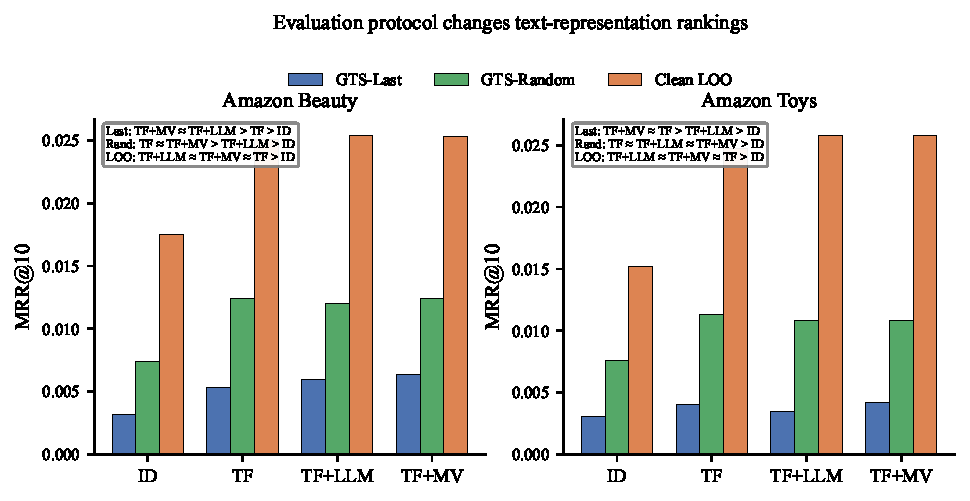
\includegraphics[width=\linewidth]{figures/fig_protocol_contrast.pdf}
\caption{%
Protocol contrast on Beauty and Toys.
GTS-Last/Random: warm MRR@10 (3 training seeds; Random further averaged over 3 target-sampling seeds).
LOO: clean leave-one-out (contrast only).
Clean LOO yields higher absolutes and favors LLM/MV; Last vs.\ Random also changes the winner among text methods.%
}
\label{fig:protocol}
\end{figure}

\begin{table}[t]
\centering
\caption{%
GTS-Last warm NDCG@10 and Hit@10 (3-seed mean$\pm$std).
Among ID/TF/LLM/MV, NDCG agrees with MRR.
UniSRec is strongest on Hit@10 (all three datasets) and on Grocery NDCG.
}
\label{tab:ndcg_hit}
\small
\setlength{\tabcolsep}{3pt}
\begin{tabular}{@{}llccccc@{}}
\toprule
Dataset & Metric & ID & TF & LLM & MV & UniSRec \\
\midrule
\multirow{2}{*}{Beauty}
 & NDCG & .0047\tiny{$\pm$.0007} & .0074\tiny{$\pm$.0006} & .0080\tiny{$\pm$.0009} & \textbf{.0087}\tiny{$\pm$.0003} & .0081\tiny{$\pm$.0003} \\
 & Hit  & .0098\tiny{$\pm$.0013} & .0146\tiny{$\pm$.0013} & .0146\tiny{$\pm$.0029} & .0167\tiny{$\pm$.0011} & \textbf{.0180}\tiny{$\pm$.0007} \\
\midrule
\multirow{2}{*}{Toys}
 & NDCG & .0046\tiny{$\pm$.0004} & .0056\tiny{$\pm$.0006} & .0046\tiny{$\pm$.0002} & .0057\tiny{$\pm$.0011} & \textbf{.0066}\tiny{$\pm$.0013} \\
 & Hit  & .0098\tiny{$\pm$.0013} & .0108\tiny{$\pm$.0011} & .0084\tiny{$\pm$.0004} & .0108\tiny{$\pm$.0027} & \textbf{.0153}\tiny{$\pm$.0030} \\
\midrule
\multirow{2}{*}{Grocery}
 & NDCG & .0048\tiny{$\pm$.0019} & .0062\tiny{$\pm$.0004} & .0063\tiny{$\pm$.0005} & .0077\tiny{$\pm$.0007} & \textbf{.0159}\tiny{$\pm$.0002} \\
 & Hit  & .0107\tiny{$\pm$.0041} & .0117\tiny{$\pm$.0009} & .0117\tiny{$\pm$.0007} & .0136\tiny{$\pm$.0007} & \textbf{.0337}\tiny{$\pm$.0005} \\
\bottomrule
\end{tabular}
\end{table}

\begin{table}[t]
\centering
\caption{%
Per-seed GTS-Last warm MRR@10 (seeds 42 / 2024 / 2026).
Variance is visible; MV's lead is small and seed-dependent.%
}
\label{tab:perseed}
\small
\setlength{\tabcolsep}{3.5pt}
\begin{tabular}{@{}llccccc@{}}
\toprule
Dataset & Seed & ID & TF & LLM & MV & UniSRec \\
\midrule
\multirow{3}{*}{Beauty}
 & 42    & .0038 & .0049 & .0063 & .0063 & .0050 \\
 & 2024  & .0032 & .0052 & .0055 & .0066 & .0054 \\
 & 2026  & .0026 & .0057 & .0063 & .0061 & .0051 \\
\midrule
\multirow{3}{*}{Toys}
 & 42    & .0033 & .0045 & .0037 & .0035 & .0044 \\
 & 2024  & .0030 & .0038 & .0032 & .0042 & .0045 \\
 & 2026  & .0029 & .0036 & .0036 & .0048 & .0031 \\
\bottomrule
\end{tabular}
\end{table}

Table~\ref{tab:protocol} and Figure~\ref{fig:protocol} present the central finding.
The key insight is \emph{not} that one text representation always wins, but that their \textbf{relative ordering is sensitive to the target-selection protocol}:

\begin{itemize}[leftmargin=*,itemsep=1pt]
\item \textbf{GTS-Last}: MV leads on all three datasets (Beauty $.0064$, Toys $.0042$, Grocery $.0058$), but the margin over LLM is small and often within one std (Table~\ref{tab:perseed}).
\item \textbf{GTS-Random} (3 sample-seed avg): TF leads on Toys ($.0113$); on Beauty TF$\approx$MV ($.0124$ / $.0124$); TF ties MV on Grocery ($.0085$).
\item \textbf{LOO}: absolute MRR is 3--6$\times$ higher than GTS-Last; ranking becomes LLM $\approx$ MV $\ge$ TF.
\end{itemize}
Last vs.\ Random is a \textbf{target-selection} effect on the same trained GTS checkpoints; LOO vs.\ GTS is a \textbf{split/training-protocol} effect (different training data and models).

\paragraph{A plausible account of the LOO gap.}
The 3--6$\times$ higher absolute scores under LOO are not merely an additive shift---they change the relative ordering among text methods.
LOO permits temporal overlap: a user's training interactions include items from the same time period as the test target, effectively allowing the model to ``memorize'' co-occurrence patterns that would not exist under a strict temporal cutoff.
A plausible explanation is that this overlap disproportionately benefits representations capturing fine-grained semantic similarity (LLM and MV), because overlapping items provide richer co-occurrence signal for semantic features than for lexical ones.
Under GTS, where training and test items are temporally disjoint, this advantage vanishes and the broader lexical coverage of \tfidf becomes competitive.

\paragraph{Why do Last and Random disagree?}
Under GTS-Last, each user's single evaluation target is their \emph{chronologically last} test interaction, which is biased toward recently popular or trending items.
Under GTS-Random, the target is uniformly sampled from the test window, drawing in a broader mix of item popularities.
Multi-view embeddings, trained to capture subtle semantic distinctions, may have an edge on the harder ``predict the very last item'' task where the target is often a recently introduced or niche item.
TF-IDF, which encodes broad lexical coverage, may instead benefit from Random's more uniform target distribution, where many targets are well-represented by title keywords.
A text representation that ``wins'' under one target mode can ``lose'' under another, even with identical model weights.

\paragraph{Implications.}
The \emph{same checkpoints} (same trained weights) produce different winners when evaluated with Last vs.\ Random target selection---a pure protocol artifact.
Claims of text-representation superiority are therefore unreliable without specifying the target mode.
All text methods consistently outperform ID-only ($+$29--100\% relative under GTS-Last, wider under Random) regardless of protocol, confirming the value of text features in general.
The most accurate summary of our data is therefore: \emph{text vs.\ ID is robust; TF vs.\ LLM vs.\ MV is protocol-sensitive}.

\paragraph{UniSRec as external baseline.}
Under identical GTS-Last + min5 + warm filter, UniSRec scores $0.0052$ (Beauty) and $0.0040$ (Toys)---between ID and TF on Beauty, and tied with TF on Toys---but dominates on Grocery ($0.0106$, nearly $2\times$ the next best).
Table~\ref{tab:ndcg_hit} shows that NDCG@10 largely agrees with MRR rankings under GTS-Last, while Hit@10 elevates UniSRec across all three datasets---a reminder that metric choice interacts with protocol.
We therefore treat MRR as the primary ranking metric and report NDCG/Hit for completeness.
Previously reported ``UniSRec wins'' arose from inconsistent evaluation filters (Appendix~\ref{app:unisrec}).
The choice of minimum interaction threshold, candidate scope (warm vs.\ full), and target mode can each independently shift the perceived ranking of an external baseline.

%==============================================================================
\section{RQ2: Temporal Robustness}
\label{sec:rq2}
%==============================================================================

\begin{table}[t]
\centering
\caption{%
Main ($80\%$ cutoff) vs.\ Early ($60\%$ cutoff) on Beauty --- GTS-Last warm MRR@10 (3-seed mean$\pm$std).
Equal-horizon TS $[0.6,0.1,0.1]$; hyperparameters frozen from Main.
The Main row matches Table~\ref{tab:protocol}.
The Early row is a temporal stress test, not yet a fully matched-protocol retrain (see text).%
}
\label{tab:early}
\small
\begin{tabular}{@{}lccc@{}}
\toprule
Window & TF & LLM & MV \\
\midrule
Main      & .0053\tiny{$\pm$.0004} & .0060\tiny{$\pm$.0004} & \textbf{.0064}\tiny{$\pm$.0003} \\
Early60-EQ & .0036\tiny{$\pm$.0007} & .0038\tiny{$\pm$.0003} & \textbf{.0043}\tiny{$\pm$.0006} \\
\bottomrule
\end{tabular}
\end{table}

\begin{table}[t]
\centering
\caption{%
Temporal distribution shift (valid$\to$test, Main GTS).
Reported as \emph{associations} with the observed Main$\to$Early performance decline, not causal claims.%
}
\label{tab:shift}
\small
\setlength{\tabcolsep}{4pt}
\begin{tabular}{@{}lccc@{}}
\toprule
Dataset & Unseen targets & Pop mean (V$\to$T) & Pop median (V$\to$T) \\
\midrule
Beauty  & 31.9\% & $112.8 \to 101.8$ & $21 \to 15$ \\
Toys    & 40.8\% & $144.7 \to 119.1$ & $18 \to 11$ \\
Grocery & 29.6\% & $87.3 \to 76.9$ & $16 \to 12$ \\
\bottomrule
\end{tabular}
\end{table}

\begin{table}[t]
\centering
\caption{%
Target popularity-bucket composition (valid$\to$test, Main GTS).
Head share drops while unseen share rises---concurrent with absolute metric degradation.%
}
\label{tab:bucket}
\small
\setlength{\tabcolsep}{3.5pt}
\begin{tabular}{@{}llcccc@{}}
\toprule
Dataset & Split & Head & Mid & Low & Unseen \\
\midrule
\multirow{2}{*}{Beauty}
 & Valid & 63.1\% & 15.9\% & 9.7\% & 11.3\% \\
 & Test  & 56.6\% & 14.9\% & 10.7\% & 17.8\% \\
\midrule
\multirow{2}{*}{Toys}
 & Valid & 60.1\% & 16.3\% & 10.6\% & 13.0\% \\
 & Test  & 52.3\% & 15.5\% & 11.0\% & 21.3\% \\
\bottomrule
\end{tabular}
\end{table}

To isolate the effect of training-window size from test-horizon length, we use an equal-horizon Early split $[0.6, 0.1, 0.1]$ that keeps valid and test at the same 10\% span as Main, sliding only the training cutoff from 80\% to 60\%.

Table~\ref{tab:early} reports GTS-Last warm MRR@10 for both windows.
The Early checkpoints use the equal-horizon split, but they additionally differ from Main in fusion defaults (cross-attention, inference boost) and catalog-fit rather than cutoff-fit embeddings; we therefore treat this comparison as a temporal stress test, not as an isolated cutoff ablation.
A matched-protocol Early retrain is in progress.
Absolute scores still drop from Main to Early across all models, with MV leading narrowly in both windows and TF, LLM, and MV remaining within 0.001 of each other.
Table~\ref{tab:shift} documents concurrent shifts in target composition: 30--41\% of test targets are items absent from training, and target popularity declines.
Table~\ref{tab:bucket} further decomposes the shift into popularity buckets: from valid to test, head share falls by $\approx$6--8 points while unseen share rises by $\approx$6--8 points on both Beauty and Toys.

\textbf{No single text variant dominates} once the temporal window is varied.

\paragraph{Connecting shift to representation type.}
Why might temporal shift interact differently with \tfidf vs.\ LLM representations?
TF-IDF, being a lexical model, is anchored to token frequencies observed during training.
When the test catalog shifts toward newer items with unfamiliar token distributions, TF-IDF's discriminative power degrades---but this degradation is \emph{uniform} across items, preserving relative rankings.
LLM embeddings, by contrast, derive their structure from a pretrained language model that generalizes to unseen text, potentially maintaining more absolute performance under catalog shift.
However, this advantage is modulated by the target-selection mode: when targets are dominated by popular items (as in Last), LLM/MV's semantic precision may help; when targets are more uniformly sampled (as in Random), the broader lexical coverage of \tfidf becomes competitive.
We emphasize association rather than causation: the shift statistics co-occur with the Main$\to$Early drop, but we do not claim that unseen share alone \emph{causes} the ranking pattern.

%==============================================================================
\section{RQ3: Why Limited Multi-View Gain}
\label{sec:rq3}
%==============================================================================

\begin{figure}[t]
\centering
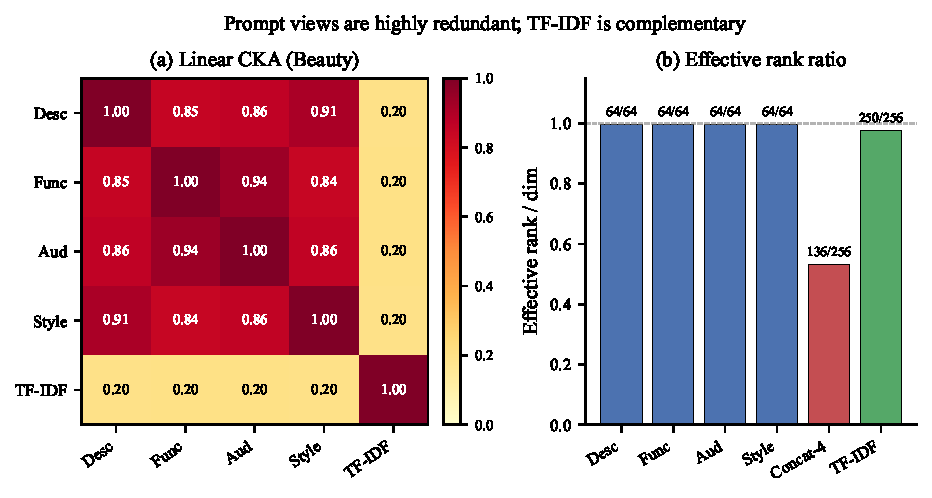
\includegraphics[width=\linewidth]{figures/fig_cka_heatmap.pdf}
\caption{%
Representation analysis on Beauty (3 random item subsamples of 3{,}000 each, mean$\pm$std).
\textbf{(a)}~Pairwise CKA: LLM views show high mutual similarity (0.84--0.94); TF--LLM CKA is low ($\approx$0.20).
\textbf{(b)}~Effective rank: 4-view concat 136/256 (53\%) vs.\ TF-IDF 250/256 (98\%).%
}
\label{fig:cka}
\end{figure}

\begin{table}[t]
\centering
\caption{%
Inter-view CKA (3 subsamples of 3K items, mean$\pm$std).
All LLM view pairs exceed 0.82; TF-IDF vs.\ any LLM view stays below 0.20.%
}
\label{tab:cka}
\small
\setlength{\tabcolsep}{4pt}
\begin{tabular}{@{}lcc@{}}
\toprule
View Pair & Beauty & Toys \\
\midrule
Description--Function  & $.846 \pm .001$ & $.834 \pm .001$ \\
Description--Audience  & $.860 \pm .001$ & $.856 \pm .002$ \\
Description--Style     & $.914 \pm .000$ & $.904 \pm .001$ \\
Function--Audience     & $.940 \pm .000$ & $.921 \pm .001$ \\
Function--Style        & $.843 \pm .001$ & $.818 \pm .002$ \\
Audience--Style        & $.859 \pm .001$ & $.838 \pm .002$ \\
\midrule
\emph{TF-IDF vs.\ LLM view (range)} & $.196$--$.201$ & $.184$--$.189$ \\
\bottomrule
\end{tabular}
\end{table}

\begin{table}[t]
\centering
\caption{%
Effective rank (Beauty/Toys, 3 subsamples).
4-view concat occupies only 53--55\% of its nominal dimensionality.%
}
\label{tab:effrank}
\small
\begin{tabular}{@{}lccc@{}}
\toprule
Representation & Dim & ER (Beauty) & ER (Toys) \\
\midrule
Single LLM view (avg) & 64 & 63.7 (99.5\%) & 63.6 (99.4\%) \\
4-view concat & 256 & 136.1 (\textbf{53.2\%}) & 141.2 (\textbf{55.2\%}) \\
TF-IDF (SVD) & 256 & 249.9 (97.6\%) & 251.4 (98.2\%) \\
\bottomrule
\end{tabular}
\end{table}

\begin{table}[t]
\centering
\caption{%
Leave-one-view-out (zero-mask, 3-seed mean).
$\Delta$: MRR@10 change vs.\ the full 4-view model.
Maximum $|\Delta|$ is 0.00035.
Absolute MRR is \emph{not} GTS-Last (recompute pending); we use only the near-zero $\Delta$ as a redundancy diagnostic.%
}
\label{tab:loov}
\small
\setlength{\tabcolsep}{3.5pt}
\begin{tabular}{@{}lccccc@{}}
\toprule
Dataset & Full MRR & $-$Desc & $-$Func & $-$Aud & $-$Style \\
\midrule
% TODO(P1): Beauty row is still RecBole-default GTS-All, not GTS-Last.
%           wrap_beauty_mv cutoff-fit exists; do not paste this-morning ~.016 md.
% Toys row VERIFIED: Aug-14 GTS-Last 3-seed mean on cutoff-fit wrap_toys_mv.
Beauty & .01571 & $-$.00021 & $+$.00005 & $-$.00002 & $-$.00017 \\
Toys   & .01089 & $-$.00035 & $-$.00011 & $-$.00015 & $-$.00033 \\
\bottomrule
\end{tabular}
\end{table}

We address RQ3 by triangulating three complementary analyses.
No single measure suffices: CKA captures structural similarity but cannot alone prove task-irrelevance~\cite{kornblith2019cka}; effective rank measures dimensionality utilization; LOOV measures downstream impact.
Together they provide converging evidence that prompt multi-view gains are limited by inter-view redundancy.

\paragraph{(1) High inter-view CKA.}
Table~\ref{tab:cka} and Figure~\ref{fig:cka}(a) show that all six LLM view pairs have CKA $\ge 0.82$ (Beauty 0.84--0.94; Toys 0.82--0.92).
The four prompt views, generated from the same encoder applied to the same item text with different instructions, encode highly similar relational structures.
In contrast, TF-IDF vs.\ any LLM view yields CKA $\approx$0.19--0.20 (Beauty) and 0.18--0.19 (Toys)---a qualitatively different regime indicating substantial representational dissimilarity.

\paragraph{(2) Pairwise cosine vs.\ CKA.}
Mean pairwise cosine between prompt views is often moderate or near zero (e.g., Description--Function $\approx -0.01$ on Beauty), while Function--Audience reaches $\approx 0.42$.
This does \emph{not} contradict high CKA: cosine measures instance-level alignment of vectors, whereas CKA compares Gram-matrix geometry across the item set~\cite{kornblith2019cka}.
Views can have low average cosine yet still induce nearly isomorphic similarity structures---precisely the failure mode of ``semantic paraphrasing'' via prompts.
We therefore treat CKA as the primary similarity diagnostic and use cosine only as a complementary check, never as standalone proof of redundancy.

\paragraph{(3) Low effective rank of concatenated views.}
Table~\ref{tab:effrank} and Figure~\ref{fig:cka}(b) show that concatenating four 64-d views into 256 dimensions yields effective rank of only 136 (Beauty) and 141 (Toys), occupying 53--55\% of the available capacity.
Nearly half the dimensions are ``consumed'' by redundant structure.
TF-IDF at the same 256-d has effective rank $\ge$250 (97--98\%), utilizing almost all capacity.
The quantitative thresholds above confirm substantial dimensionality collapse in multi-view concatenation.

\paragraph{(4) Negligible LOOV impact.}
Table~\ref{tab:loov} shows that zeroing any single view has minimal downstream effect: maximum $|\Delta|$ = 0.00035.
A GTS-Last warm recompute is pending, so we do \emph{not} treat the absolute Full MRR in that table as a main-protocol ranking result; the diagnostic we retain is that dropping any one view barely moves the score.

\paragraph{Where does redundancy originate?}
To disentangle prompt-induced from preprocessing-induced redundancy, we compare CKA at two stages: \emph{pre-whitening} (SVD-projected + centered, 64-d per view, \textbf{without} ZCA whitening) and \emph{post-whitening} (the final model-input embeddings).
On Beauty, mean pairwise CKA is $0.96\pm0.001$ pre-whitening and $0.87\pm0.001$ post-whitening; on Toys, $0.96\pm0.001$ and $0.86\pm0.001$ respectively.
CKA is \emph{already extremely high before whitening} (Table~\ref{tab:cka-prepost})---whitening actually \emph{reduces} inter-view CKA by $\sim$0.09 and increases concatenated effective rank from 99/256 (39\%) to 136/256 (53\%) on Beauty (similarly 104$\to$140 on Toys).

To trace redundancy further upstream, we compute inter-view CKA directly on the raw 3584-d Qwen hidden states \emph{before any SVD projection}.
Mean pairwise CKA at 3584-d is $0.961$ on Beauty and $0.963$ on Toys (3-trial random subsample of 3000 items, $\sigma < 0.002$).
Effective rank of the concatenated 4-view matrix ($4\times 3584 = 14336$-d) is only 1567 (10.9\%) on Beauty and 1622 (11.3\%) on Toys.
Redundancy is therefore \textbf{inherent in the Qwen encoder's representations}, not an artifact of SVD truncation: the LLM produces near-isomorphic relational structures regardless of the instruction prompt, and the $\sim$90\% dimensionality collapse is already present at the source.
Whitening partially decorrelates the views but cannot remove this structural overlap.
Expanding view dimensionality to $4\times256$ is thus \emph{not} justified---the bottleneck is source redundancy, not projection capacity (Table~\ref{tab:cost}).

\begin{table}[t]
\centering
\caption{%
Pre- vs.\ post-whitening audit (3 item-subsamples, mean).
CKA is already $\ge$0.94 before whitening; whitening lowers CKA and raises concat effective rank, so redundancy is not a whitening artifact.%
}
\label{tab:cka-prepost}
\small
\begin{tabular}{@{}llcc@{}}
\toprule
Dataset & Stage & Pairwise CKA & Concat ER/256 \\
\midrule
\multirow{2}{*}{Beauty}
 & Pre-whiten (SVD+center)  & 0.94--0.99 & 99 (39\%) \\
 & Post-whiten (TS fit)     & 0.84--0.94 & 136 (53\%) \\
\midrule
\multirow{2}{*}{Toys}
 & Pre-whiten (SVD+center)  & 0.94--0.98 & 104 (41\%) \\
 & Post-whiten (TS fit)     & 0.82--0.92 & 140 (55\%) \\
\bottomrule
\end{tabular}
\end{table}

\paragraph{Synthesis.}
All three diagnostics point in the same direction: prompt views encode overlapping semantics, leading to dimensionality collapse and negligible per-view contribution.
This is consistent with multi-view theory---views derived from a single source via semantic paraphrasing fail the complementarity condition~\cite{xu2013multiview}.
The potential complementarity in our system lies between lexical \tfidf and semantic \llm (CKA$\approx$0.19), suggesting representational dissimilarity that is not harvested by naive multi-prompt stacking---the MV model simply replicates similar semantic structures four times instead of combining lexical and semantic axes.

%==============================================================================
\section{Discussion and Limitations}
\label{sec:discussion}
%==============================================================================

\paragraph{Why does TF-IDF match multi-view LLM?}
Why can a bag-of-words representation match or exceed four LLM views under GTS-Random?
Two factors act in combination.
First, \tfidf captures \emph{lexical diversity}: the vocabulary of product titles and descriptions spans tens of thousands of unique tokens, and SVD-projected TF-IDF retains nearly all available capacity (ER/dim $\approx$0.98; Table~\ref{tab:effrank}).
Each dimension contributes distinct information.
Second, the four LLM views suffer from \emph{semantic homogeneity}: because the same pretrained encoder processes the same item text with only minor instruction changes, the resulting representations share highly similar relational geometry (CKA 0.82--0.94).
Concatenating four such views nominally quadruples dimensionality but effectively adds only $\sim$50\% new capacity.
Put differently, TF-IDF does not capture richer semantics than an LLM, but its \emph{geometric diversity per dimension} is far higher.
Under GTS protocols where distribution shift makes fine-grained semantic distinctions less reliable (Table~\ref{tab:shift}), this geometric diversity becomes a practical advantage.

\paragraph{Pure LLM-only ablation.}
To verify that TF-IDF features do not merely act as a ``free init'' for the LLM head, we train a variant using only a single Qwen2.5-7B view with \emph{no} TF-IDF base (same architecture, same two-phase pipeline).
Under the main protocol (GTS-Last warm, min5, train-catalog candidates), this variant scores $.0046\pm.0001$ on Beauty and $.0018\pm.0007$ on Toys---below the TF-anchored LLM column in Table~\ref{tab:protocol} ($.0060$ / $.0035$) and below ID-only on Toys.
We therefore do \emph{not} conclude that a pure LLM embedding matches the standard LLM pipeline.

\paragraph{TF+LLM hybrid ablation.}
To test whether the lexical--semantic dissimilarity identified in RQ3 (TF--LLM CKA$\approx$0.19) translates into additive gains, we train a hybrid using the MV architecture with \tfidf base and a single LLM view (no extra prompt views).
This comparison is reserved for GTS-Last and GTS-Random on saved checkpoints---the same target modes as Table~\ref{tab:protocol}---not GTS-All validation.
A matched-protocol hybrid retrain was paused to finish the Early-window experiment; until GTS-Last/Random numbers from that retrain are available we withhold ranking claims.
Low TF--LLM CKA licenses only \emph{geometric dissimilarity}; whether the two families are additive on next-item ranking is left to that evaluation.

\paragraph{Practitioner implications.}
\begin{enumerate}[leftmargin=*,itemsep=2pt]
\item Report text-representation comparisons under GTS with explicit target mode.  LOO can reverse rankings and yield 3--6$\times$ higher absolute metrics.
\item Start with cutoff-fit \tfidf as a strong baseline.  Under GTS-Random it ties or leads MV; under GTS-Last it is competitive but may trail LLM/MV.  Given its negligible preprocessing cost relative to LLM inference, TF-IDF should be the first text baseline evaluated.
\item A single \llm view typically matches four prompt views; diagnose redundancy (e.g., via CKA and effective rank) before investing in multi-view pipelines.
\item Adding more prompt views from the same encoder yields negligible gains.  Geometric diversity between representation families (lexical \tfidf vs.\ semantic \llm) is a more plausible complementarity axis than extra prompts, but additive ranking gains must be verified under GTS-Last/Random rather than assumed from low CKA or from GTS-All validation scores.
\item Do not overclaim a single ``best'' text representation across protocols; report Last and Random (or Successive) side by side, as rankings can reverse between target modes.
\end{enumerate}

\paragraph{Limitations.}
\begin{itemize}[leftmargin=*,itemsep=1pt]
\item \textbf{Warm-target scope.}
Our models lack content-only zero-shot fallback; warm-target evaluation is thus the fairest comparison, but it excludes 30--41\% of real test items.
\item \textbf{Static metadata.}
We use fixed product titles/descriptions; temporally evolving text (e.g., reviews, trending tags) could change the TF/LLM balance.
\item \textbf{Amazon-only domain.}
All three datasets are Amazon subcategories.  Grocery is a same-platform replication, not a solution to domain diversity.
\item \textbf{GTS-Random reproducibility.}
We average GTS-Random over three target-sampling seeds (42, 123, 456).  Cross-seed standard deviation of warm MRR@10 per checkpoint is 0.001--0.003, indicating moderate but non-negligible sensitivity to target sampling~\cite{gusak2025time}.
\item \textbf{Redundancy locus.}
Our redundancy audit now spans three stages---raw 3584-d Qwen hidden states, 256-d SVD-projected, and 64-d post-whitening---confirming that view collapse originates in the encoder itself (Section~\ref{sec:rq3}).  However, only a single LLM (Qwen2.5-7B) is tested; other architectures may exhibit different inter-view structure.
\item \textbf{Successive not fully run.}
We rely on Last/Random as proxies; a sampled-user Successive sanity check would further validate protocol choice.
\end{itemize}

\paragraph{Cost analysis.}
\begin{table}[t]
\centering
\caption{Parameter count and inference cost (seed~42).  MV adds $<$1\% parameters.}
\label{tab:cost}
\small
\begin{tabular}{@{}lcc@{}}
\toprule
Model & Params (M) & ms/sample \\
\midrule
ID / TF / LLM / MV & 67.2 / 67.4 / 67.6 / 67.7 & 0.02 \\
UniSRec & 67.7 & 0.04 \\
\bottomrule
\multicolumn{3}{@{}l}{\footnotesize Beauty; Toys is $\sim$87M due to larger vocab (ranking identical).}
\end{tabular}
\end{table}

Table~\ref{tab:cost} confirms multi-view failure is not a capacity issue.  All variants have effectively the same parameter budget and inference cost.

%==============================================================================
\section{Conclusion}
\label{sec:conclusion}
%==============================================================================

We conducted a leakage-aware controlled study of text representations for sequential recommendation, structured as an empirical investigation rather than a model-proposal paper.
Three conclusions emerge for the community:

\begin{enumerate}[leftmargin=*,itemsep=1pt]
\item \textbf{Protocol matters.}
The relative ordering of \tfidf, single-view \llm, and prompt multi-view depends on the GTS target mode.
Text features consistently outperform ID-only, but which text is best requires specifying the evaluation protocol.
Under GTS-Last, multi-view leads narrowly; under GTS-Random, \tfidf ties or leads---a reversal driven entirely by target selection, not by model changes.
\item \textbf{No text variant is consistently dominant.}
Under an equal-horizon Early window ($60\%$ cutoff, same valid/test span as Main), treated here as a temporal stress test, absolute MRR drops substantially but text variants remain within 0.001 of each other; the Main-window pattern of near-ties persists.
The most honest summary of the data is that text helps, but which text helps most is an evaluation artifact as much as a representation property.
\item \textbf{Multi-view gains are limited by inter-view redundancy.}
CKA, effective rank, and LOOV jointly show that prompt views encode overlapping semantics; potential complementarity lies between lexical and semantic features (CKA$\approx$0.19), not between different prompt instructions applied to the same encoder.
Whether a TF+LLM hybrid converts that dissimilarity into ranking gains is evaluated under GTS-Last/Random on saved checkpoints, not assumed from CKA or from GTS-All validation.
\end{enumerate}

Text-enhanced sequential recommendation is increasingly treated as an LLM upgrade problem---more parameters, more prompts, and more views are assumed to monotonically improve quality.
Our evidence suggests the community should first lock the temporal protocol, then diagnose representation redundancy, before investing in additional prompt views or fusion modules.
The practical default under leakage-aware evaluation is: report GTS-Last (and Random as a check), keep cutoff-fit \tfidf as a mandatory baseline, and treat multi-view LLM features as a hypothesis to be tested---not a free upgrade.

\paragraph{Future directions.}
We outline five open questions.
(1)~\textbf{Scalable hybrid TF+LLM fusion.}  Whether lexical--semantic fusion yields additive gains under GTS-Last/Random (the main protocol) remains open; more sophisticated fusion (e.g., gating, cross-attention) is a natural follow-up.
(2)~\textbf{Cross-architecture redundancy audit.}  Our raw 3584-d audit confirms the redundancy locus in Qwen2.5-7B.  Testing whether the same inter-view collapse holds for decoder-only vs.\ encoder-only LLMs (e.g., Mistral, BERT-large) would clarify whether this is a general transformer property or specific to the Qwen family.
(3)~\textbf{GTS-Successive evaluation} at sampled-user scale, to validate Last/Random as proxies for online next-item prediction~\cite{gusak2025time}.
(4)~\textbf{Non-Amazon domains} with reliable timestamps, to test whether protocol sensitivity generalizes beyond product catalogs.
(5)~\textbf{Instruction-diverse prompts} that enforce semantic divergence (e.g., attribute extraction vs.\ sentiment summarization) to test whether complementarity can be engineered at the prompt level.

\section*{Ethical Considerations}
This work uses public Amazon review datasets with no personally identifiable attributes beyond standard user/item IDs.
Potential concerns include reinforcing popularity bias under temporal shift and inheriting biases from LLM-generated text features.
We mitigate the former by reporting warm-target stratified diagnostics and the latter by treating multi-view LLM features as an empirical object of study rather than a recommended default.
No human subjects were involved.

\begin{acks}
Anonymous for review.
\end{acks}

%==============================================================================
\appendix
%==============================================================================

\section{GTS-All Results}
\label{app:gts-all}

Main tables use GTS-Last (one last target per user).
GTS-All evaluates all post-cutoff targets (Beauty: 4{,}520 users $\to$ 12{,}001 samples, avg 2.65/user; Toys: 4{,}873 users $\to$ 13{,}186, avg 2.71/user).

\begin{table}[h]
\centering
\caption{GTS-All warm MRR@10 (3-seed mean).  TF dominates under All.}
\label{tab:gts-all}
\small
\begin{tabular}{@{}lccccc@{}}
\toprule
Dataset & ID & TF & LLM & MV & UniSRec \\
\midrule
Beauty & .0156 & \textbf{.0242} & .0236 & .0236 & .0123 \\
Toys   & .0118 & \textbf{.0191} & .0181 & .0184 & .0082 \\
\bottomrule
\end{tabular}
\end{table}

Under GTS-All, TF is unambiguously strongest---broadly aligning with GTS-Random (where TF leads or ties MV) but diverging from GTS-Last.
Per \citet{gusak2025time}, All has the lowest rank-correlation with Successive and introduces task mismatch, which is why we relegate it to appendix.

\section{Grocery Per-Seed Breakdown}
\label{app:grocery}

\begin{table}[h]
\centering
\caption{Grocery warm MRR@10 per seed under GTS-Last and GTS-Random.}
\label{tab:grocery-perseed}
\small
\setlength{\tabcolsep}{3pt}
\begin{tabular}{@{}llcccc@{}}
\toprule
Protocol & Seed & ID & TF & LLM & MV \\
\midrule
\multirow{3}{*}{GTS-Last}
 & 42    & .0027 & .0038 & .0049 & .0052 \\
 & 2024  & .0019 & .0049 & .0050 & .0058 \\
 & 2026  & .0043 & .0050 & .0041 & .0065 \\
\midrule
\multirow{3}{*}{GTS-Rand}
 & 42    & .0038 & .0069 & .0073 & .0084 \\
 & 2024  & .0036 & .0093 & .0085 & .0079 \\
 & 2026  & .0058 & .0093 & .0078 & .0093 \\
\bottomrule
\end{tabular}
\end{table}

Grocery replicates the Beauty/Toys pattern under the same search budget: MV leads narrowly on Last; TF and MV are competitive on Random.
We treat it as same-platform replication, not a domain-diversity claim.

\section{GTS-Random Target-Sampling Seeds}
\label{app:random-seeds}

Main-table GTS-Random numbers average three target-sampling seeds $\{42,123,456\}$ on the same checkpoints (no retraining).
Table~\ref{tab:random-seeds} reports each seed after averaging the three training seeds.
Cross-seed std of warm MRR@10 is typically 0.001--0.003; seed~456 is systematically lower, which is why a single Random seed would overstate TF's Beauty lead (0.0138 vs.\ 3-seed 0.0124).

\begin{table}[h]
\centering
\caption{GTS-Random warm MRR@10 by target-sampling seed (mean over training seeds 42/2024/2026).}
\label{tab:random-seeds}
\small
\setlength{\tabcolsep}{3pt}
\begin{tabular}{@{}llccccc@{}}
\toprule
Dataset & Sample seed & ID & TF & LLM & MV & UniSRec \\
\midrule
\multirow{3}{*}{Beauty}
 & 42    & .0081 & .0138 & .0133 & .0134 & .0098 \\
 & 123   & .0080 & .0134 & .0128 & .0141 & .0103 \\
 & 456   & .0063 & .0101 & .0099 & .0098 & .0087 \\
\midrule
\multirow{3}{*}{Toys}
 & 42    & .0096 & .0146 & .0140 & .0141 & .0103 \\
 & 123   & .0066 & .0091 & .0089 & .0085 & .0078 \\
 & 456   & .0065 & .0101 & .0095 & .0098 & .0075 \\
\bottomrule
\end{tabular}
\end{table}

\section{All-Target and Cross-Attention}
\label{app:alltarget}

\paragraph{All-target evaluation.}
Including unseen test items (absent from train catalog) decreases absolute MRR uniformly but preserves ranking order.
Unseen-target shares: Beauty 31.9\%, Toys 40.8\%, Grocery 29.6\%.
Without content-only zero-shot capability, all models score near-zero on unseen items; warm-target scope is the fairest comparison.

\paragraph{Cross-attention (negative result).}
\label{app:cross}
A sequence-level cross-attention module attending to text-view features was tested but improves and degrades per-user performance roughly equally; it is excluded from the main method.

\section{UniSRec Detailed Results}
\label{app:unisrec}

UniSRec~\cite{hou2022unisrec} was initially evaluated without the \texttt{min\_train\_inter}=5 filter, yielding higher MRR@10 (Beauty 0.0204--0.0208; Toys 0.0162--0.0164).
After applying the same filter:

\begin{table}[h]
\centering
\small
\begin{tabular}{@{}lccc@{}}
\toprule
Dataset & GTS-All & GTS-Last & GTS-Random$^\dagger$ \\
\midrule
Beauty & .0123$\pm$.0001 & .0052$\pm$.0002 & .0096$\pm$.0001 \\
Toys   & .0082$\pm$.0001 & .0040$\pm$.0008 & .0085$\pm$.0003 \\
\bottomrule
\end{tabular}
\end{table}

\noindent$^\dagger$GTS-Random averaged over target-sampling seeds $\{42,123,456\}$ (same protocol as Table~\ref{tab:protocol}).

Under fair comparison, UniSRec sits between ID and TF on Beauty MRR and ties TF on Toys, consistent with its use of a single LLM view without the alignment warmup that benefits our LLM/MV variants.
On Hit@10 under GTS-Last, UniSRec is stronger (Table~\ref{tab:ndcg_hit}), suggesting backbone differences affect metrics differently.

\bibliographystyle{ACM-Reference-Format}
\bibliography{refs_0819}

\end{document}
